\documentclass{article}
\usepackage[T1]{fontenc}
\usepackage{lmodern}
\usepackage{graphicx}
\usepackage{amsmath,amssymb}
\usepackage[a4paper,margin=2cm]{geometry}
\usepackage[absolute,overlay]{textpos}
\setlength{\TPHorizModule}{1mm}
\setlength{\TPVertModule}{1mm}
\usepackage[indonesian]{babel}
\usepackage{hyperref}
\setlength{\emergencystretch}{2em}
% unit: Halaman 50

\begin{document}

% === Halaman 50 (llm) ===

\vspace{243.54mm}

def dekripsi\_aes(cipherteks, kunci):
    kunci = kunci.encode()
    cipherteks = base64.b64decode(cipherteks)
    iv = cipherteks[:16]
    AEScipher = AES.new(kunci, AES.MODE\_CBC, iv)
    plainteks = AEScipher.decrypt(cipherteks[BLOCK\_SIZE:])
    plainteks = unpad(plainteks, BLOCK\_SIZE)
    return plainteks

def encrypt\_file(input\_file, output\_file, key):
    with open(input\_file, 'rb') as f:
        plaintext = f.read()

    ciphertext = enkripsi\_aes(plaintext, key)

    with open(output\_file, 'wb') as f:
        f.write(ciphertext)

def decrypt\_file(input\_file, output\_file, key):
    with open(input\_file, 'rb') as f:
        ciphertext = f.read()

    plaintext = dekripsi\_aes(ciphertext, key)

    with open(output\_file, 'wb') as f:
        f.write(plaintext)

% deskripsi: Screenshot potongan kode Python untuk implementasi enkripsi dan dekripsi file menggunakan algoritma AES.
% bbox normalisasi: [0.0600, 0.0600, 0.8800, 0.8800]
\begin{textblock*}{172.20mm}(12.60mm,17.82mm)
\noindent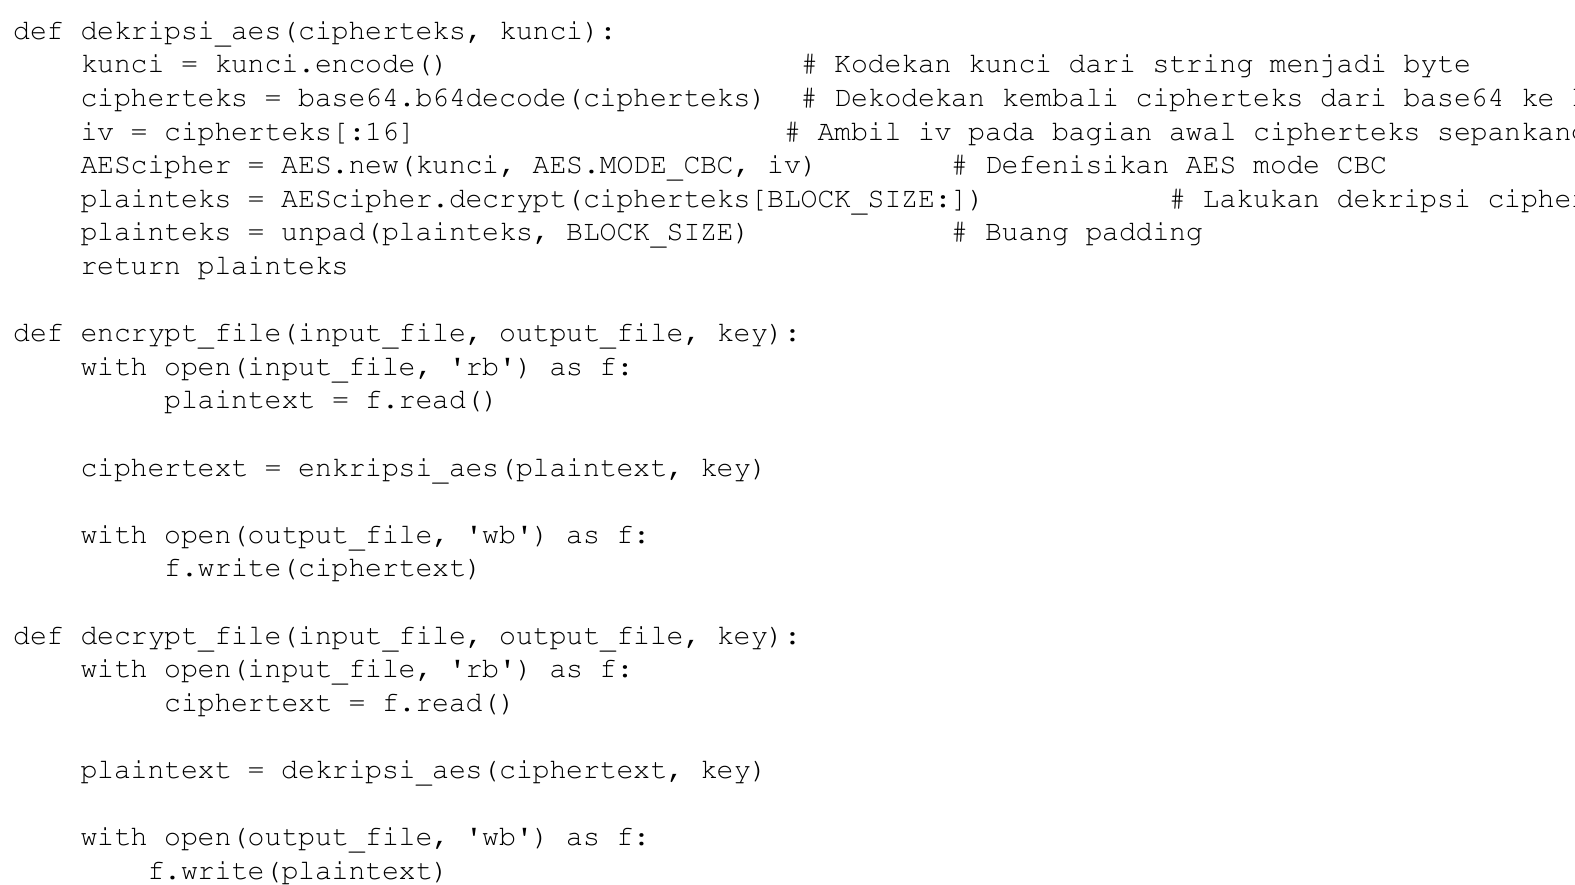
\includegraphics[width=172.20mm,height=243.54mm]{../../images/llm/page_050_img_01.png}%
\end{textblock*}

\end{document}
